\textbf{¿Cuál es el \'area del triángulo de la figura \ref{fig:area_isoseles_01}?}

\begin{figure}[H]
    \centering
    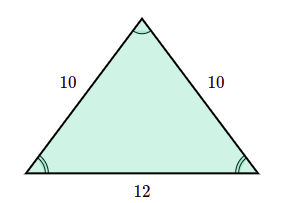
\includegraphics[width=0.25\textwidth]{../images/area_isoseles_01.png}
    \caption{}
    \label{fig:area_isoseles_01}
\end{figure}

\begin{solutionbox}{15cm}
    \begin{figure}[H]
        \centering\captionsetup[subfigure]{justification=centering}
        \begin{subfigure}{0.25\linewidth}
            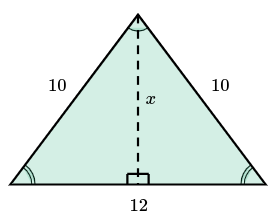
\includegraphics[width=\linewidth]{../images/area_isoseles_01a.png}
            \caption{}
            \label{subfig:area_isoseles_01a}
        \end{subfigure}
        \begin{subfigure}{0.25\linewidth}
            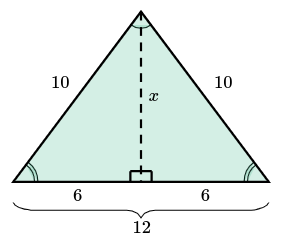
\includegraphics[width=\linewidth]{../images/area_isoseles_01b.png}
            \caption{}
            \label{subfig:area_isoseles_01b}
        \end{subfigure}
    \end{figure}
    Para determinar el área del triángulo debemos saber la base y la altura. Llamemos $x$ a la altura (ver Figura \ref{subfig:area_isoseles_01a}).
    Estos dos triángulos rectángulos son congruentes porque uno es la reflexión del otro a través de la línea punteada.
    La base de cada triángulo rectángulo es la mitad de la base del triángulo isósceles.
    Cuando tenemos un triángulo rectángulo, podemos usar el teorema de Pitágoras para obtener la altura (ver Figura \ref{subfig:area_isoseles_01b}).
    La ecuación para el teorema de Pitágoras es:
    \[c^2=a^2+b^2\]
    En este caso, $a=6$, $b=x$ y $c=10$. Entonces,
    \begin{align*}
        6^2+x^2 & =10^2   \\
        36+x^2  & =100    \\
        x^2     & =100-36 \\
        x^2     & =64     \\
        x       & =8
    \end{align*}
    La altura del triángulo es 8.
    El área del triángulo es
    \[A=\frac{1}{2}\cdot 12 \cdot 8 = 48 \text{ u}^2\]
\end{solutionbox}